\section{Metodologia}

O presente projeto tem a intenção de desenvolver um sistema \acs{\acs{CNN}}, que será formado a partir de uma arquitetura de \acs{IA} híbrida, em que uma parte desse modelo terá a tarefa de lidar com a base de dados de imagens que será fornecida pela \ac{FMABC}, sendo essa base composta de imagens de pacientes brasileiros afetados pela psoríase, e a outra parte lidar com os dados clínicos, como por exemplo exames de sangue PCR e velocidade de hemossedimentação, ambos os exames podem sofrer alteração em casos inflamatórios, que também será fornecido pela \acs{FMABC} em anuência do comitê de ética em pesquisa da \acs{FMABC}. A intenção dessa proposta é que a combinação de diferentes análises e informações traga um aumento na precisão desse tipo de sistema, fornecendo um suporte à tomada de decisão. Efetivamente, será implementada uma solução de ponta a ponta, que exigirá desde técnicas para o tratamento e preparo dos dados, até soluções para o refinamento do modelo de \acs{IA}.


A partir dos conceitos de redes neurais artificiais e \textit{transformers}, fica mais claro entender a construção dos modelos de \acs{IA}, que seguem um certo padrão, esse padrão é conhecido como \textit{pipeline}. Os \textit{pipelines} de \acs{IA} envolvem todo o fluxo de atividades necessárias para o funcionamento apropriado do modelo. De modo genérico, este fluxo geralmente começa com atividades relacionadas à extração, transformação e carregamento dos dados, processo conhecido como \ac{ETL}; no caso de modelos de \acs{IA} voltados a visão computacional, essa fase utiliza técnicas para preparar essas imagens a um modelo de \acs{IA}, geralmente envolvendo atividades relacionadas ao processamento digital de imagens. Além das transformações nas imagens é necessário realizar uma estratificação dos dados, uma parte deve ser separada para o treinamento da rede, enquanto a outra deve ser exclusivamente voltada para a validação da rede. A etapa seguinte envolve o treinamento da rede, essa etapa exige diferentes técnicas para o sucesso do modelo, entre essas técnicas estão a escolha de um algoritmo de otimização adequado ao problema, o uso de uma função de perda apropriada, ajuste correto dos hiperparâmetros da rede e número de épocas no treinamento.

Foram estudadas diversas alternativas de parametrização da rede proposta com o objetivo de aumentar a precisão dos diagnósticos, dentre as técnicas aplicadas, se destaca o \textit{GridSearch} . O pipeline desse projeto pode ser dividido inicialmente em algumas etapas, começando com a construção de uma aplicação para a extração, transformação e carregamento (\acs{ETL}) dos dados, em que, serão realizadas todas as atividades necessárias para garantir que esses dados estejam seguros e disponíveis, seguindo com técnicas de aumento da base de dados de imagens para o treinamento do modelo de \acs{CNN}, esta fase irá exigir um estudo profundo do conjunto de dados de imagens, pois as transformações aplicadas nas imagens terão impacto direto em como a \acs{CNN} irá desempenhar futuramente. Transformações como o tamanho da imagem, conversão de domínio de cores, rotação das imagens, entre outras diversas transformações serão avaliadas neste momento. Essas técnicas também possibilitam que o modelo seja treinado com uma base de dados maior e mais diversificada, aumentando sua generalização. Além da aplicação de técnicas de aumento da base será necessário utilizar metodologias para a estratificação dos dados, o método utilizado será de validação cruzada k-pastas estratificado para avaliar o desempenho do modelo. Em seguida, será realizado o desenvolvimento e treinamento de um modelo de \acs{CNN}, nesta fase serão estudadas diversas arquiteturas de redes convolucionais e aplicações dessas arquiteturas na área da saúde, além de alternativas para equilibrar a precisão do modelo e sua quantidade de parâmetros, um dos fatores que determina o impacto computacional da rede neural. Por fim, o modelo será avaliado utilizando diferentes métodos estatísticos, como z-score, acurácia, precisão, sensibilidade, especificidade e perda.

Já a segunda parte compõe a construção e treinamento de um modelo de \acs{MLP}, que trabalhará em conjunto com a \acs{CNN}, portanto, a saída da \acs{CNN} irá compor um dos parâmetros de entrada no \acs{MLP}. Será necessário integrar uma rede \acs{MLP} ao modelo de classificação de imagens. Além das técnicas já previstas como validação cruzada e avaliação do modelo, também será necessário analisar e tratar os dados clínicos e construir a integração dos dois modelos. Será realizado um estudo com os resultados de desempenho desses modelos de forma individual e dos modelos em conjunto, além de uma avaliação da viabilidade para a preparação de tal sistema em um produto.
%
% %\begin{table}[h!]
\centering
\setlength{\arrayrulewidth}{0.8pt}
\setlength{\tabcolsep}{5pt}
\renewcommand{\arraystretch}{1.2}


\small
\centering\begin{tabular}{|p{9cm}|*{11}{c|}}
\hline
\textbf{Atividades} & \multicolumn{11}{c|}{\textbf{Meses}} \\
\hline
  &
\textbf{1} & \textbf{2} & \textbf{3} & \textbf{4} & \textbf{5} & \textbf{6} & \textbf{7} & \textbf{8} & \textbf{9} & \textbf{10} & \textbf{11} \\ 
\hline
Criação de uma pipeline de dados para o armazenamento e tratamento dos dados & x & x &   &   &   &   &   &   &   &   &   \\ \hline
Análise detalhada das técnicas em sistemas CAD                              &   & x &   &   &   &   &   &   &   &   &   \\ \hline
Construção de uma prova de conceito do modelo de CNN para avaliar a viabilidade das técnicas escolhidas &   & x &   &   &   &   &   &   &   &   &   \\ \hline
Análise dos resultados da prova de conceito do modelo e definição das técnicas para a construção do modelo &   &   & x &   &   &   &   &   &   &   &   \\ \hline
Construção do modelo de CNN                                                &   &   &   & x & x &   &   &   &   &   &   \\ \hline
Avaliação do modelo de CNN e ajuste de hiperparâmetros                     &   &   &   &   & x & x &   &   &   &   &   \\ \hline
Construção da prova de conceito de um modelo de MLP                        &   &   &   &   &   & x &   &   &   &   &   \\ \hline
Análise de resultados da prova de conceito do modelo de MLP e definição das técnicas para o desenvolvimento do modelo de MLP &   &   &   &   &   &   & x &   &   &   &   \\ \hline
Construção do modelo MLP                                                   &   &   &   &   &   &   & x & x &   &   &   \\ \hline
Testes com o modelo e ajustes de hiperparâmetros                           &   &   &   &   &   &   &   & x & x &   &   \\ \hline
Análise de precisão do modelo em relação ao modelo de CNN                  &   &   &   &   &   &   &   &   & x & x &   \\ \hline
Análise de viabilidade do sistema                                          &   &   &   &   &   &   &   &   &   & x &   \\ \hline
Elaboração de artigo científico com apresentação dos resultados            &   &   &   &   &   &   &   &   &   & x & x \\ \hline
Processo de submissão do artigo científico para periódico                  &   &   &   &   &   &   &   &   &   &   & x \\ \hline
\end{tabular}
\caption{Cronograma de atividades do desenvolvimento do projeto.}
\label{cronograma}
\end{table}




%
% Presente projeto tem característica quantitativa, visto que se enquadra nas definições de ser conseguido na busca de resultados exatos evidenciados por meio de variáveis preestabelecidas, em que se verifica e explica a influência sobre as variáveis, mediante análise da frequência de incidências e correlações estatísticas \cite{michelmetodologia}.
%
% O desenvolvimento do trabalho se divide em duas grandes áreas de atuação, Inteligência artificial, que atende todo o escopo do desenvolvimento do modelo de segmentação. E engenharia de software, que engloba os conteúdos necessários para o desenvolvimento do protótipo de software.
%
% \subsection{Do desenvolvimento do modelo}
%
% Conforme apresentado na seção anterior, a aplicação das técnicas de visão computacional na medicina tem se mostrado muito promisoras para o diagnóstico de doenças complexas e melhora na eficiência do diagnóstico clínico. A integração de diferentes dados, como exames laboratoriais e imagens médicas, possibilitará a construção de um sistema robusto, capaz de analisar diferentes tipos e grandes volumes de dados. A Figura \ref{fig:pipeline} ilustra, de forma abstrata, como será o funcionamento do sistema proposto.
%
% \begin{figure}[h]
%     \centering
%     
\includegraphics[scale=0.15]{images/pipeline2.png}
%     \caption{Pipeline do projeto}
%     \label{fig:pipeline}
% \end{figure}
%
% Cada fase do pipeline será projetada para realizar operações críticas para o resultado do modelo, buscando também maior desempenho e resiliência para esse sistema. Serão detalhadas cada uma das etapas.
%
% \subsubsection{Coleta dos dados}
%
% Essa etapa é responsável pela extração e organização dos dados, serão utilizadas técnicas de engenharia de dados para garantir que todo o processo de coleta dos dados seja seguro e consistente. Desta maneira, para assegurar esses objetivos, o sistema terá integração com dados de diversas fontes diferentes, essa integração para a coleta das informações será feita através de interfaces de programação de aplicação (\textit{API}), que possibilitará a automatização dessa fase. Para o desenvolvimento dessa etapa, serão empregadas a linguagem de programação python e a ferramenta \textit{spark} como recursos principais. No contexto deste estudo, a coleta foi realizada a partir de bancos de dados públicos médicos, o portal escolhido responsável pelas informações é o The Cancer Imaging Archive \cite{cancerimaging}, foram extraídos diferentes conjuntos de dados. 
%
% A figura \ref{fig:ex-dataset}, apresenta uma imagem retirada do conjunto fornecido pelo the Cancer Imaging Archive. Esse conjunto é composto por 610 imagens microscópicas de melioma múltiplo. A localização do câncer é nos ossos, as imagens possuem ampliação de 1000x, tendo as dimensões de 1126x874 pixels.
%
%
% \begin{figure}[h] % Ajuste largura
%     \centering
%     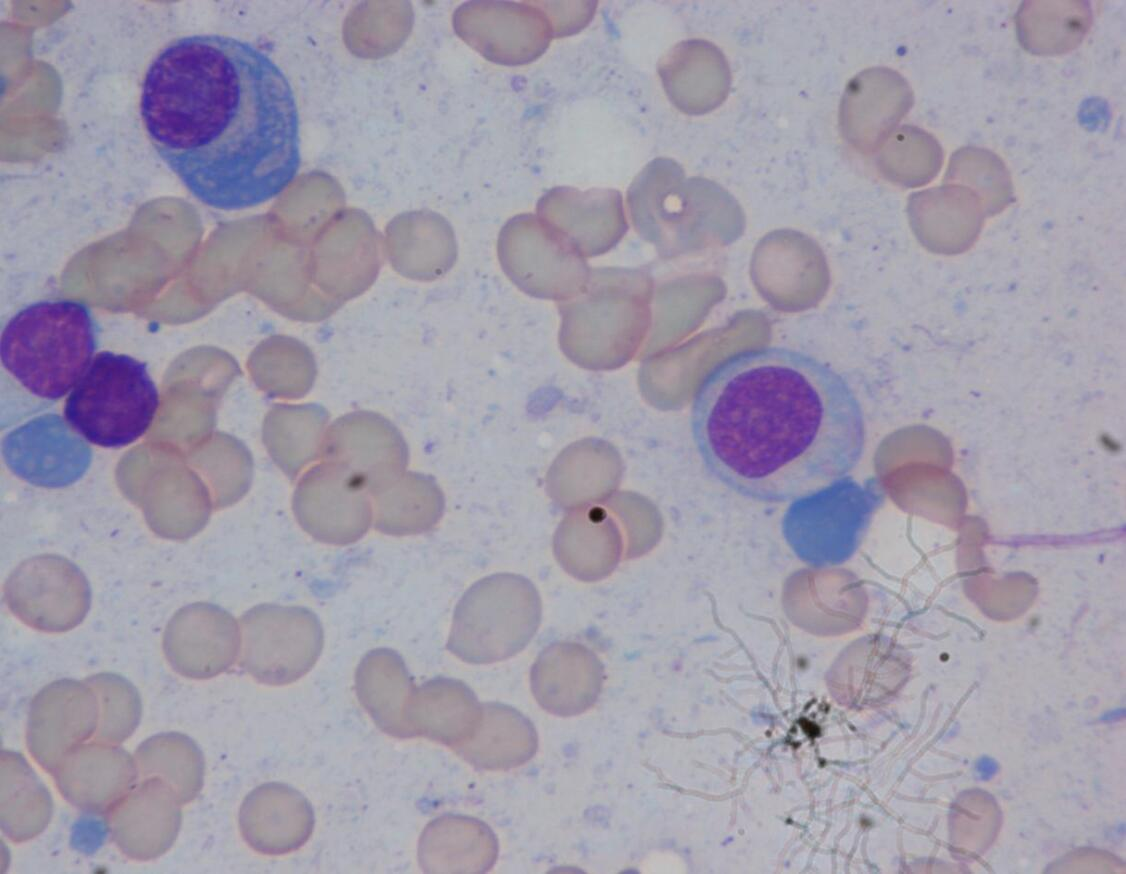
\includegraphics[width=0.3\textwidth]{images/datasetexample.jpg}
%     \caption{Imagem microscópica de câncer nos ossos}
%     \label{fig:ex-dataset}
% \end{figure}
%
% \subsubsection{Pré processamento}
%
% Após a etapa anterior, será necessário tratar as informações coletadas. Com isso, será aplicado operações como a limpeza de dados, que envolve a remoção de valores inconsistentes, ajuste de escalas de valores e codificação de variáveis categóricas, por exemplo. Além disso, para os dados de imagens, serão utilizadas técnicas de aumento de dados, para maior generalização do modelo. Também serão explorados técnicas de processamento digital de imagens, como regulagem de luminosidade e transformação para diferentes domínios de cor como YCbCr.
%
% \subsubsection{Extração de características}
%
% Antes de realizar o treinamento efetivo do modelo, será necessário extrair características a partir das imagens médicas, como textura, bordas e padrões. Durante a fase de extração de características, o principal objetivo é transformar os dados recebidos em representações que melhor capturam os padrões subjacentes e são mais informativas para o algoritmo de aprendizado. Para a seleção de características relevantes, técnicas como análise de correlação e análise de variância serão utilizados para apoio à seleção. Para os dados de imagens, a extração de características estará incorporada ao treinamento, visto que as camadas convolucionais têm a responsabilidade de aprender os padrões hierárquicos e abstratos.
%
% \subsubsection{Treinamento do modelo}
%
% Com todas as informações já preparadas, serão exploradas diferentes técnicas de convoluções para a segmentação das imagens microscópicas, como por exemplo a \textit{pixel-wise convolution}, uma técnica que possibilita a combinação de informações entre os canais de uma imagem. Será avaliado a possibilidade de utilizar técnicas de \textit{ensemble} nessa fase, de modo a combinar da melhor maneira os dados clínicos com as imagens microscópicas. Também será explorado técnicas para otimizar o treinamento, como ajuste da taxa de aprendizado de forma dinâmica entre as diferentes camadas de acordo com algumas métricas, como o erro das previsões. Para fins de melhora no desempenho, o treinamento do modelo também envolverá técnicas de computação paralela, com isso será possível um treinamento mais otimizado do sistema.
%
% \subsubsection{Avaliação do modelo}
%
% Como etapa final, a avaliação do modelo é responsável por aplicar métodos estatísticos para consolidar os resultados das etapas previstas. Conforme os resultados desses métodos, será possível analisar se o desempenho do modelo está de acordo com o esperado. Dentre as técnicas mais comuns, serão utilizadas métricas como acurácia, definida pela fórmula 
% \begin{equation}
%   acurácia = \frac{VP +VN}{VP + FN + VN + FP} \; ,
%     \label{eq: acuracia}
% \end{equation}
% \\
% em que \(VP\) é a quantidade de verdadeiros positivos; \(VN\) é a quantidade de verdadeiros negativos; \(FN\) é a quantidade de falsos negativos e \(FP\) é a quantidade de falsos positivos. Também será utilizado a métrica de avaliação precisão, determinada pela fórmula:
%
% \begin{equation} 
%   precisão = \frac{VP}{VP + VF} \; ,
%   \label{eq: precisao}
% \end{equation}
%  \\
% E por último, uma métrica de avaliação chamada sensibilidade, estabelecida pela fórmula:
%
% \begin{equation}
% sensibilidade = \frac{VP}{VP + FN} \; ,
%   \label{eq: sensibilidade}
% \end{equation}
% \\
% Paralelamente, todas as fases irão contar com um minucioso registro de todas as ações para monitoramento do sistema. Além disso, serão implementados mecanismos de auditoria para garantir a rastreabilidade das operações realizadas, promovendo maior transparência e confiabilidade. Esse registro incluirá não apenas informações sobre as decisões tomadas pelo sistema, mas também os dados utilizados em cada etapa, possibilitando a análise detalhada de possíveis erros ou inconsistências e facilitando ajustes futuros para otimização do desempenho.
%
% \subsection{Do protótipo da aplicação web}
%
% Para o uso desse modelo em um potencial sistema, serão utilizados diferentes componentes de tecnologia, envolvendo áreas como arquitetura de software, desenvolvimento backend, computação em nuvem, e conceitos de computação distribuída, a fim de projetar um sistema que seja resiliente, distribuído e escalável.
%
% \subsubsection{Da arquitetura do protótipo}
% O sistema proposto adota uma arquitetura baseada em microsserviços, modelo arquitetural que promove o desacoplamento dos componentes, permitindo evolução independente de cada serviço. Essa abordagem facilita a escalabilidade horizontal, melhora a manutenção e possibilita a implementação de diferentes tecnologias conforme as necessidades específicas de cada módulo. Além disso, a divisão funcional dos serviços contribui para um gerenciamento mais eficiente da infraestrutura e do processamento de dados, garantindo maior flexibilidade e modularidade no desenvolvimento e na implantação.
%
% \subsubsection{Da definição dos protocolos de comunicação}
% Além da definição da arquitetura desse protótipo, também serão explorados protocolos de comunicação de alta desempenho para garantir maior confiabilidade e reduzir latência entre os serviços. Protocolos como o \textit{Remote Procedure Call} (RPC) serão utilizados para garantir essa comunicação eficiente entre serviços. O RPC possui algumas vantagens em relação a outros protocolos, dentre elas estão a serialização binária e suporte a conexões persistentes, características que garantem um \textit{payload} menor sendo trafegado, reduzindo a latência e otimizando o desempenho \cite{Niswar2024}. 
%
% \subsubsection{Do monitoramento do protótipo}
% A fim de avaliar o desempenho do sistema proposto, serão implementadas estratégias de monitoramento para análise detalhada do comportamento da aplicação em diferentes cenários de carga e uso. Ferramentas como Prometheus e Grafana serão empregadas para coleta de métricas e visualização do desempenho dos microsserviços em tempo real, permitindo identificação de potenciais gargalos e otimizações. Além disso, serão adotadas técnicas de observabilidade avançadas, como logs estruturados e rastreamento distribuído com OpenTelemetry, possibilitando uma análise aprofundada das interações entre os serviços e assegurando uma resposta eficiente a eventuais falhas.
%
% % --- Poderia ficar nos objetivos? ---
% % Além do desenvolvimento de um modelo que seja capaz de segmentar imagens microscópicas de células com alta precisão, esse trabalho também propõe a aplicação desse modelo num sistema destinado a uso médico. 

